% 对偶空间：伴随与特殊线性算子。

\section{伴随与特殊线性算子}
\label{sec:ls-adjoints}
对偶映射把输出端的读取$f$传回输入端，得到读取$f\circ T$。若把两端的读取都换成表示它的向量，就得到伴随。
\begin{definition}[伴随]
\label{def:linear-algebra-adjoint}
设$T:V\to W$是两个有限维实内积空间之间的线性映射。若存在$T^\star:W\to V$使
\begin{equation}
 \langle T\bm x,\bm y\rangle_W=\langle\bm x,T^\star\bm y\rangle_V
 \label{eq:ls-adjoint-pairing}
\end{equation}
对所有$\bm x\in V$、$\bm y\in W$成立，则$T^\star$称为$T$的\term{伴随}（adjoint）。
\end{definition}

伴随总存在且唯一。固定$\bm y\in W$，$\bm x\mapsto\langle T\bm x,\bm y\rangle_W$是$V$上的线性泛函。由定理~\ref{thm:ls-riesz-representation}，存在唯一的向量使它写成与该向量的内积，把这个向量记为$T^\star\bm y$。$T^\star$对$\bm y$线性：
\[
 \langle\bm x,aT^\star\bm y+bT^\star\bm y'\rangle_V=a\langle T\bm x,\bm y\rangle_W+b\langle T\bm x,\bm y'\rangle_W=\langle T\bm x,a\bm y+b\bm y'\rangle_W,
\]
由表示向量的唯一性，$T^\star(a\bm y+b\bm y')=aT^\star\bm y+bT^\star\bm y'$。

用对偶映射的语言说，把$\bm y\in W$看成读取$\langle\cdot,\bm y\rangle_W$，则$T'$把它送到读取$\langle T\,\cdot,\bm y\rangle_W=\langle\cdot,T^\star\bm y\rangle_V$。所以伴随就是借内积把读取换成向量以后的对偶映射。

具体计算时，取$V,W$的基。由坐标下的内积公式，两边的内积写成$\langle\bm x,\bm x'\rangle_V=\bm x^\top\bm M_V\bm x'$、$\langle\bm y,\bm y'\rangle_W=\bm y^\top\bm M_W\bm y'$，这里$\bm x,\bm y$等指坐标，$\bm M_V,\bm M_W$是两组基的Gram矩阵，对称正定因而可逆。设$T$的矩阵为$\bm A$，伴随的矩阵为$\bm B$。式~\eqref{eq:ls-adjoint-pairing}要求$(\bm A\bm x)^\top\bm M_W\bm y=\bm x^\top\bm M_V\bm B\bm y$对所有$\bm x,\bm y$成立。取$\bm x,\bm y$为标准坐标向量逐个比较元素，这等价于$\bm A^\top\bm M_W=\bm M_V\bm B$，即
\begin{equation}
 \bm B=\bm M_V^{-1}\bm A^\top\bm M_W.
 \label{eq:ls-weighted-adjoint}
\end{equation}
两端都取标准正交基时，$\bm M_V,\bm M_W$都是单位矩阵，伴随矩阵就是$\bm A^\top$，与对偶映射的矩阵相同。一般情形下，伴随既不是单纯转置，也不是转置再求逆。下面的例子说明这一点。
\begin{example}[加权内积下的伴随]
\label{ex:ls-weighted-adjoint}
设$V=W=\mathbb R^2$都取加权内积$\langle\bm x,\bm y\rangle_{\bm M}=\bm x^\top\bm M\bm y$，$\bm M=\operatorname{diag}(4,1)$，并考虑把第二个坐标移到第一个位置的映射$T\bm x=\bm A\bm x$，其中
\[
 \bm A=\begin{bmatrix}0&1\\0&0\end{bmatrix}.
\]
标准基在这个内积下不是标准正交基，所以伴随要用式~\eqref{eq:ls-weighted-adjoint}计算：
\[
 \bm B=\bm M^{-1}\bm A^\top\bm M
 =\begin{bmatrix}1/4&0\\0&1\end{bmatrix}\begin{bmatrix}0&0\\1&0\end{bmatrix}\begin{bmatrix}4&0\\0&1\end{bmatrix}
 =\begin{bmatrix}0&0\\4&0\end{bmatrix}.
\]
再回到配对等式核对：$\bm A\bm x=(x_2,0)^\top$，$\langle\bm A\bm x,\bm y\rangle_{\bm M}=4x_2y_1$；$\bm B\bm y=(0,4y_1)^\top$，$\langle\bm x,\bm B\bm y\rangle_{\bm M}=x_2\cdot4y_1$，两者相等。因数$4$来自输出落在权重为$4$的第一个坐标上，伴随要把这个权重带回输入端。所以伴随矩阵是$\bm B$，而不是$\bm A^\top$：
\[
 \bm B=\begin{bmatrix}0&0\\4&0\end{bmatrix}\neq\begin{bmatrix}0&0\\1&0\end{bmatrix}=\bm A^\top.
\]
\end{example}
对偶映射的矩阵总是$\bm A^\top$；伴随与它的差别，来自读取与向量之间的对应$\bm a\mapsto\bm M^{-1}\bm a$随内积改变。四个基本子空间正交关系的证明只用到配对恒等式，所以在一般内积空间中同样有$\ker T^\star=(\operatorname{im}T)^\perp$、$\ker T=(\operatorname{im}T^\star)^\perp$。

\paragraph{伴随的运算规则}
由配对定义可以逐条推出伴随的运算规则：
\[
 \begin{gathered}
(T+S)^\star=T^\star+S^\star,\\
(cT)^\star=c\,T^\star,\\
(TS)^\star=S^\star T^\star,\\
T^{\star\star}=T.
 \end{gathered}
\]
例如$\langle TS\bm x,\bm y\rangle=\langle S\bm x,T^\star\bm y\rangle=\langle\bm x,S^\star T^\star\bm y\rangle$，复合的伴随与乘积的转置一样反转次序；恒等映射的伴随是自身。图~\ref{fig:ls-adjoint-action-transfer}画出伴随怎样把配对从输出端搬回输入端。

伴随不是逆：逆把输出复原成输入，伴随只把作用从内积的一侧移到另一侧。
\begin{example}[反例：伴随不是逆]
\label{ex:ls-adjoint-not-inverse}
最简单的反例是非零内积空间$V$上的放大两倍$T=2\operatorname{id}$。数乘可以从内积的一侧移到另一侧，$\langle2\bm x,\bm y\rangle=\langle\bm x,2\bm y\rangle$对一切$\bm x,\bm y$成立，所以$T^\star=2\operatorname{id}$：伴随仍是放大两倍。复原输入的逆却是缩小一半，$T^{-1}=\tfrac12\operatorname{id}$。因此$T^\star\neq T^{-1}$。两者相等恰好是正交算子的条件，下面马上会遇到。
\end{example}
\begin{figure}[!htb]
  \centering
  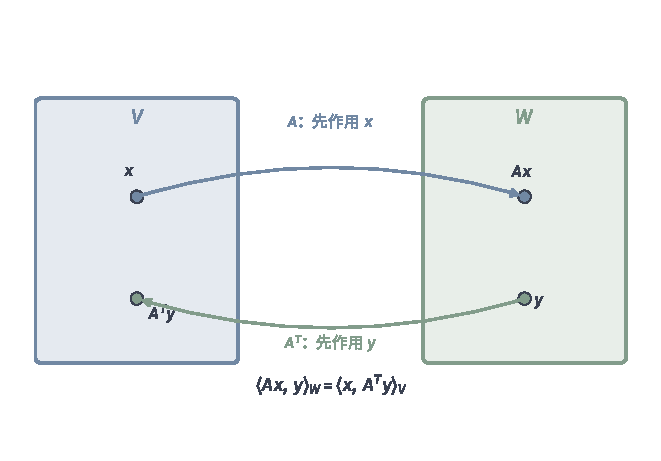
\includegraphics[width=112mm]{figures/00-shared/mathematical-preliminaries-upper/02-linear-spaces/matplotlib/ls-adjoint-action-transfer/ls-adjoint-action-transfer.pdf}
  \caption{内积伴随把输出端的配对搬回输入端。左：$T:V\to W$把$\bm x$映成$T\bm x$，与$\bm y\in W$配对；右：伴随$T^\star:W\to V$把$\bm y$映回$T^\star\bm y\in V$，使$\langle T\bm x,\bm y\rangle_W=\langle\bm x,T^\star\bm y\rangle_V$。标准欧氏内积下$T^\star$就是转置；它反转的是配对的方向，不是逆作用。箭头与空间为解析示意。}
  \label{fig:ls-adjoint-action-transfer}
\end{figure}

\paragraph{自伴、正交与正规算子}
对算子$T:V\to V$，伴随仍是$V$上的算子，可以与$T$比较。下面四类算子都由$T$与$T^\star$之间的一个等式规定。

若$T^\star=T$，称$T$为\term{自伴}（self-adjoint）算子，它在标准正交基下对应对称矩阵。若$T^\star=-T$，称$T$为\term{反自伴}（skew-adjoint）算子，它在标准正交基下对应满足$\bm A^\top=-\bm A$的反对称矩阵。反自伴算子把每个向量送到与它正交的方向：由$\langle T\bm x,\bm x\rangle=\langle\bm x,T^\star\bm x\rangle=-\langle\bm x,T\bm x\rangle$得$\langle T\bm x,\bm x\rangle=0$。例如平面上的$\left[\begin{smallmatrix}0&-1\\1&0\end{smallmatrix}\right]$把$(x_1,x_2)^\top$送到$(-x_2,x_1)^\top$，即逆时针旋转直角。

若$Q^\star Q=\operatorname{id}$，则$Q$保持内积：$\langle Q\bm x,Q\bm y\rangle=\langle\bm x,Q^\star Q\bm y\rangle=\langle\bm x,\bm y\rangle$，称为正交算子。它在标准正交基下对应第~\ref{sec:ls-orthogonal-matrices}节的正交矩阵；由方阵的单侧逆即双侧逆，$Q^{-1}=Q^\star$。

满足$TT^\star=T^\star T$的算子称为\term{正规}（normal）算子，即$T$与自己的伴随可交换。自伴、反自伴与正交算子都是正规算子：前两种情形$T^\star=\pm T$显然与$T$交换，正交算子满足$QQ^\star=Q^\star Q=\operatorname{id}$。一般算子未必正规，例如示例~\ref{ex:ls-weighted-adjoint}中的$\bm A=\left[\begin{smallmatrix}0&1\\0&0\end{smallmatrix}\right]$在欧氏内积下满足$\bm A\bm A^\top=\operatorname{diag}(1,0)\neq\operatorname{diag}(0,1)=\bm A^\top\bm A$。这些算子的谱性质在第~\ref{chap:eigen-spectral-decomposition}章讨论，这里只给出定义。

\paragraph{复空间中的泛函表示与伴随}
复空间沿用前面“第一变量共轭线性、第二变量线性”的约定。这时线性泛函应写成$\varphi(\bm x)=\langle\bm v,\bm x\rangle$，让$\bm x$处于线性的变量位置。若$\bm q_1,\ldots,\bm q_d$是标准正交基，则$\bm v=\sum_j\overline{\varphi(\bm q_j)}\bm q_j$；代入各基向量即可核对读数。表示向量随泛函作共轭线性变化，这与实空间中的线性对应不同。

例如在$\mathbb C$的标准内积$\langle v,z\rangle=\overline v z$下，泛函$\varphi(z)=(1+\mathrm i)z$对应$v=1-\mathrm i$，因为$\overline v z=(1+\mathrm i)z$。若交换两个变量的位置，得到的表达式关于$z$共轭线性，不再是线性泛函。所以共轭来自内积约定，不能从实数公式中直接删去。

两个复内积空间之间的伴随仍由$\langle T\bm x,\bm y\rangle_W=\langle\bm x,T^\star\bm y\rangle_V$定义。在标准正交基下，若$T$的矩阵为$\bm A$，伴随的矩阵就是$\bm A^*$；若两端基的Gram矩阵为$\bm M_V,\bm M_W$，则为$\bm M_V^{-1}\bm A^*\bm M_W$。这与代数对偶映射的矩阵$\bm A^\top$不同：后者只复合线性泛函，不涉及内积和共轭。复空间中，自伴矩阵满足$\bm A=\bm A^*$；保持内积的方阵满足$\bm A^*\bm A=\bm I$，称为酉矩阵。
